
\section{Experimental Results}
We have written some scripts for some basic graph plotting and some analysis.\\
Below is one of the experimental result.\\
\begin{figure}[!ht]
	\centering
	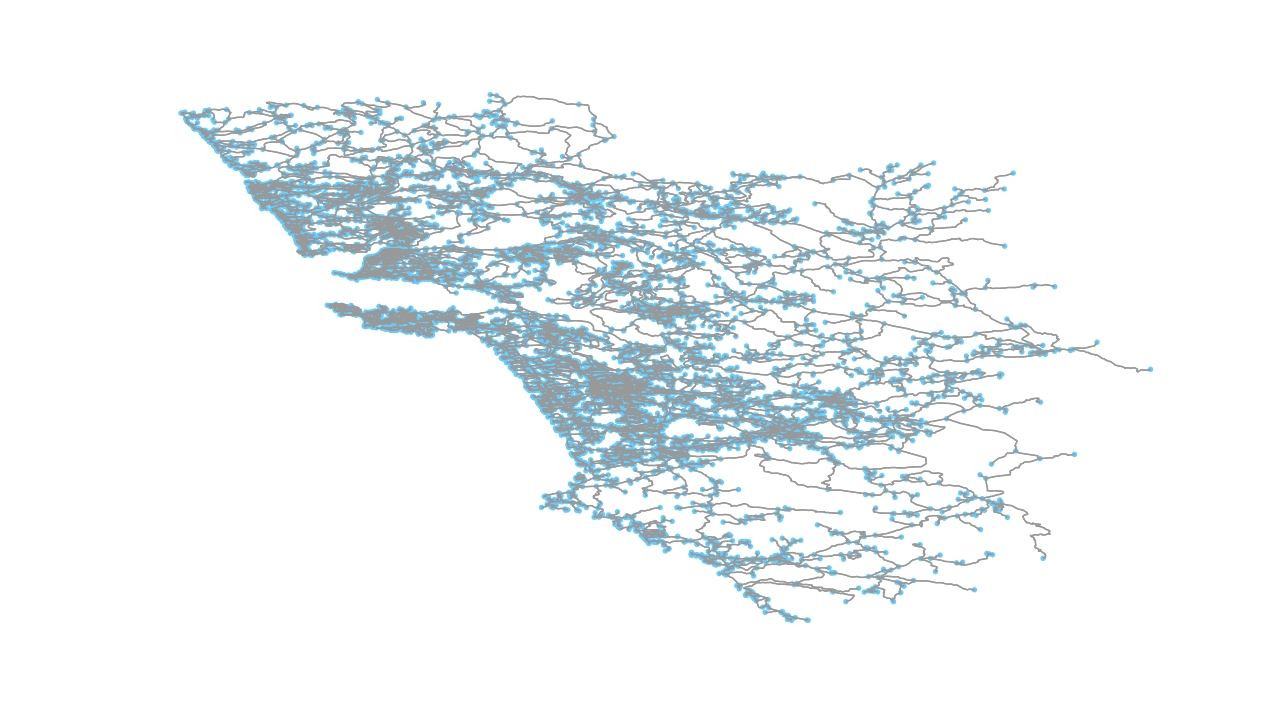
\includegraphics[width=0.7\textwidth]{input/images/plot1.jpg}              
	\caption{Goa Road Network Plotted}
	\hspace{-1.5em}
\end{figure}\\
You may refer to my blogs also for detailed information.\\
Here is the url: \\
http://geoffboeing.com/ \\\\
Road network of Punjab looks like this:
\begin{figure}[!ht]
	\centering
	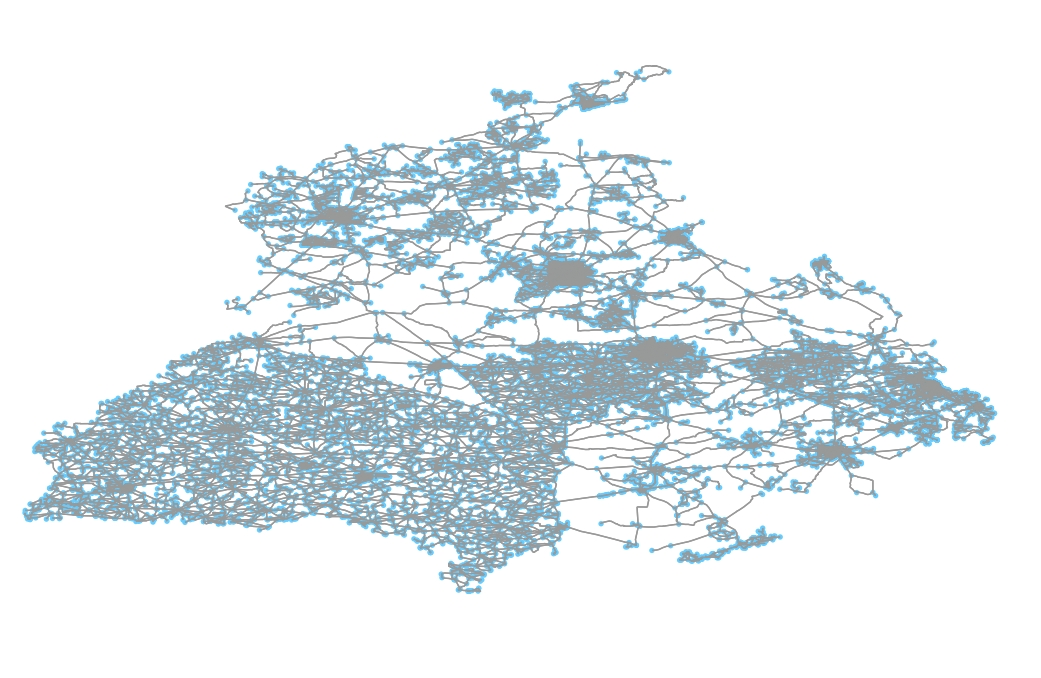
\includegraphics[width=0.7\textwidth]{input/images/p.jpg}                
	\caption{Punjab road network}
	\hspace{-1.5em}
\end{figure}\\\\
\subsubsection{Create Road Networks}
Script to create road networks

\begin{description}
	
	\item [\ import osmnx as ox]\\
	\item [\ T ="#Place osm tag here"]
	\item [\ ox.plot\_graph(ox.graph\_from\_place(T))]\\
	
\end{description}

\subsubsection{Create Road Networks}
Script result for finding pagerank using NetworkX:

\begin{figure}[!ht]
	\centering
	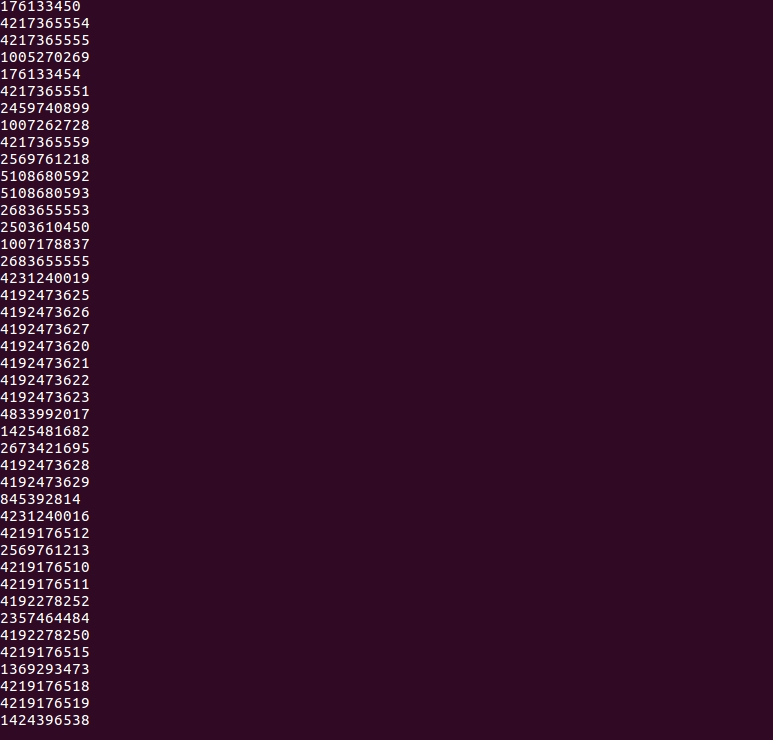
\includegraphics[width=0.7\textwidth]{input/images/pg.jpg}              
	\caption{Pagerank using NetworkX}
	\hspace{-1.5em}
\end{figure}\\

\subsubsection{Create Road Networks}
Script result for finding pagerank using GraphFrames:

\begin{figure}[!ht]
	\centering
	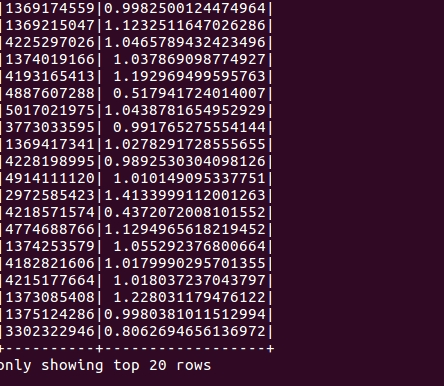
\includegraphics[width=0.7\textwidth]{input/images/pggf.jpg}              
	\caption{Pagerank using GraphFrames}
	\hspace{-1.5em}
\end{figure}\\
 
\section{Conclusions}
We concluded some information using processing times and other analysis as follows:  
\subsection{When to use NetworkX}
\begin{itemize}
	\item Unlike many other tools, it is designed to handle data on a scale relevant to
	modern problems.
	\item Most of the core algorithms rely on extremely fast legacy code
	\item Highly flexible graph implementations (a graph/node can be anything!)
	\item Extensive set of native readable and writable formats
	\item Takes advantage of Python’s ability to pull data from the Internet or databases
\end{itemize}
\subsection{When not to use NetworkX}
\begin{itemize}
	\item Large-scale problems that require faster approaches (i.e. massive networks
	with 100M/1B edges)
	\item Better use of memory/threads than Python (large objects, parallel computation)
\end{itemize}
 

